\documentclass{article}
\usepackage[a4paper,margin=2.5cm]{geometry}
\usepackage{amsmath}
\usepackage{tikz}
\usetikzlibrary{calc,arrows.meta}

\begin{document}

\section*{Trapesium Sama Kaki yang Jujur pada Kesejajarannya}

Trapesium dengan sisi sejajar $b=12$, $a=8$, dan tinggi $t=6$. Kesejajaran
dijamin lewat koordinat: titik $D$ dan $C$ sama-sama berada di $y=6$, titik
$A$ dan $B$ di $y=0$.

\begin{center}
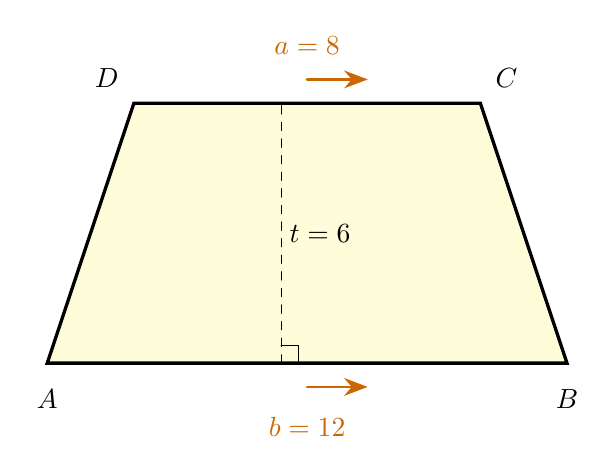
\begin{tikzpicture}[x=0.55cm,y=0.55cm,line cap=round]
  \coordinate (A) at (0,0);
  \coordinate (B) at (12,0);
  \coordinate (C) at (10,6);
  \coordinate (D) at (2,6);

  \fill[yellow!15] (A) -- (B) -- (C) -- (D) -- cycle;
  \draw[very thick] (A) -- (B) -- (C) -- (D) -- cycle;

  % tinggi
  \draw[dashed] ($(A)!0.45!(B)$) -- ++(0,6);
  \node at ($(A)!0.45!(B)+(0.9,3)$) {$t=6$};
  \draw ($(A)!0.45!(B)+(0.4,0)$) -- ($(A)!0.45!(B)+(0.4,0.4)$) -- ($(A)!0.45!(B)+(0,0.4)$);

  % panah kesejajaran
  \draw[-{Stealth[length=3mm]},orange!80!black,line width=1pt]
    ($(A)!0.5!(B)+(0,-0.55)$) -- ($(A)!0.5!(B)+(1.4,-0.55)$);
  \draw[-{Stealth[length=3mm]},orange!80!black,line width=1pt]
    ($(D)!0.5!(C)+(0,0.55)$) -- ($(D)!0.5!(C)+(1.4,0.55)$);

  \node[below=6pt] at (A) {$A$};
  \node[below=6pt] at (B) {$B$};
  \node[above right=2pt] at (C) {$C$};
  \node[above left=2pt] at (D) {$D$};
  \node[below=16pt,orange!80!black] at ($(A)!0.5!(B)$) {$b=12$};
  \node[above=14pt,orange!80!black] at ($(D)!0.5!(C)$) {$a=8$};
\end{tikzpicture}
\end{center}

\section*{Trapesium yang Diputar tetap Sejajar}

Gambar yang sama dalam tiga orientasi berbeda. Pasangan sisi sejajarnya
tidak berubah --- kesejajaran adalah sifat antara dua garis, bukan sifat
posisi alas.

\begin{center}
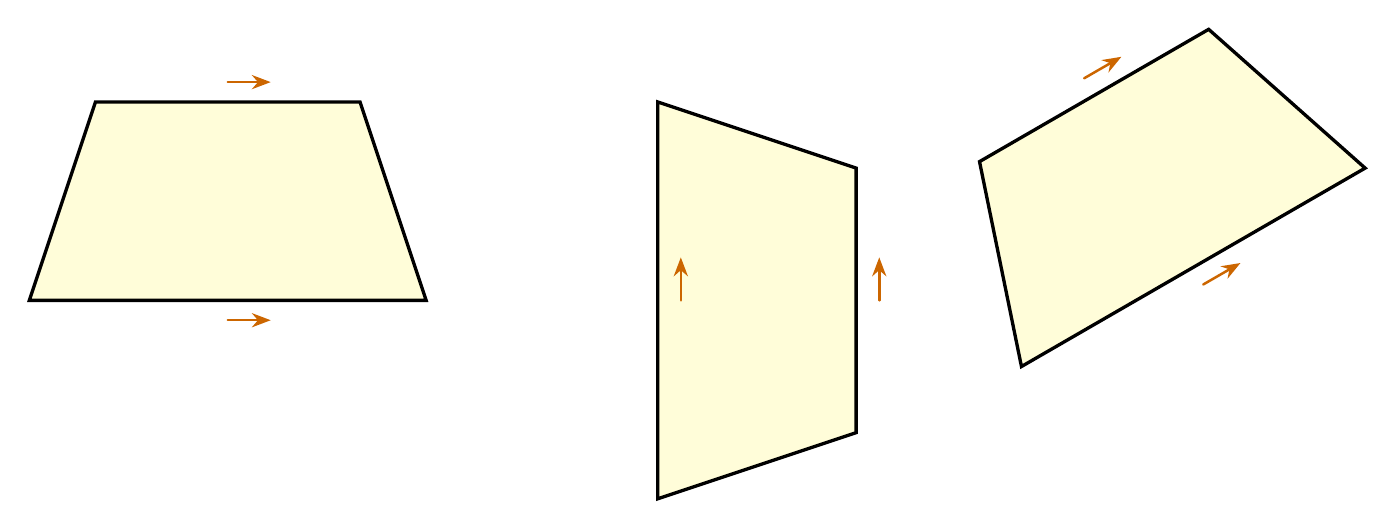
\begin{tikzpicture}[x=0.42cm,y=0.42cm,line cap=round]
  \def\trap{ (0,0) -- (12,0) -- (10,6) -- (2,6) -- cycle }

  \begin{scope}[shift={(0,0)}]
    \fill[yellow!15] \trap;
    \draw[very thick] \trap;
    \draw[-{Stealth[length=2.4mm]},orange!80!black,line width=0.9pt]
      ($(0,0)!0.5!(12,0)+(0,-0.6)$) -- ($(0,0)!0.5!(12,0)+(1.3,-0.6)$);
    \draw[-{Stealth[length=2.4mm]},orange!80!black,line width=0.9pt]
      ($(2,6)!0.5!(10,6)+(0,0.6)$) -- ($(2,6)!0.5!(10,6)+(1.3,0.6)$);
  \end{scope}

  \begin{scope}[shift={(19,6)},rotate=-90]
    \fill[yellow!15] \trap;
    \draw[very thick] \trap;
    \draw[-{Stealth[length=2.4mm]},orange!80!black,line width=0.9pt]
      ($(0,0)!0.5!(12,0)+(0,0.7)$) -- ($(0,0)!0.5!(12,0)+(-1.3,0.7)$);
    \draw[-{Stealth[length=2.4mm]},orange!80!black,line width=0.9pt]
      ($(2,6)!0.5!(10,6)+(0,0.7)$) -- ($(2,6)!0.5!(10,6)+(-1.3,0.7)$);
  \end{scope}

  \begin{scope}[shift={(30,-2)},rotate=30]
    \fill[yellow!15] \trap;
    \draw[very thick] \trap;
    \draw[-{Stealth[length=2.4mm]},orange!80!black,line width=0.9pt]
      ($(0,0)!0.5!(12,0)+(0,-0.6)$) -- ($(0,0)!0.5!(12,0)+(1.3,-0.6)$);
    \draw[-{Stealth[length=2.4mm]},orange!80!black,line width=0.9pt]
      ($(2,6)!0.5!(10,6)+(0,0.6)$) -- ($(2,6)!0.5!(10,6)+(1.3,0.6)$);
  \end{scope}
\end{tikzpicture}
\end{center}

\section*{Catatan Koordinat}

Sisi miring (kaki) trapesium: pergeseran horizontal 2 satuan dan vertikal
6 satuan, sehingga panjangnya $\sqrt{2^2+6^2}=\sqrt{40}\approx 6{,}32$
satuan. Luas trapesium:
\[
L=\frac{(a+b)}{2}\cdot t=\frac{(8+12)}{2}\cdot 6=60 \text{ satuan luas.}
\]

\end{document}
